% !TeX program = lualatex

\documentclass[12pt]{article}



\usepackage[margin=1in]{geometry} 
\usepackage{amsmath,amsthm,amssymb}
\usepackage{MnSymbol}
\usepackage{graphicx}
\usepackage{bm}
\usepackage[normalem,normalbf]{ulem}
\usepackage{algorithm} 
\usepackage{algpseudocode} 
\usepackage{multirow}
\usepackage{rotating}
\usepackage{therefore}

\usepackage{tikz}
\usetikzlibrary{shapes.multipart}
\usetikzlibrary{shapes.symbols}

\usetikzlibrary{graphs,graphdrawing,graphs.standard,quotes}
\usegdlibrary{circular,force,layered,routing}
\tikzset{
	graphs/simpleer/.style={
		nodes={draw,circle, blue, left color=blue!20, text=black, inner sep=1pt},
		node distance=2.5cm, nodes={minimum size=2em}
	},
	every loop/.style={},
}

\newcommand*\circled[1]{\tikz[baseline=(char.base)]{
		\node[shape=circle,draw,inner sep=2pt] (char) {#1};}}

\newcommand{\m}{\medskip\\}
\newcommand{\N}{\mathbb{N}}
\newcommand{\Z}{\mathbb{Z}}
\newcommand{\R}{\mathbb{R}}
\newcommand{\bbs}{\textbackslash\textbackslash\space}
\newcommand{\bs}{\textbackslash\space}
\newcommand{\la}{\enskip\land\enskip}
\newcommand{\lo}{\enskip\lor\enskip}
\newcommand{\comp}[1]{#1^\mathsf{c}}
\newcommand{\micdrop}{\qed}
\newcommand{\contra}{\begin{tikzpicture}
		\node[starburst, draw, minimum width=3cm, minimum height=2cm,line width=1.5pt,red,fill=yellow,scale=.5]
		{BOOM, A CONTRADICTION!!!};
\end{tikzpicture}}

\renewcommand{\qedsymbol}{$\blacksquare$}

\DeclareMathOperator{\lcm}{lcm}

\newtheorem{theorem}{Theorem}

\newenvironment{exercise}[2][Exercise]{\begin{trivlist}
		\item[\hskip \labelsep {\bfseries #1}\hskip \labelsep {\bfseries #2.}]}{\end{trivlist}}

\setlength\parindent{24pt}

\makeatletter
\renewcommand*\env@matrix[1][*\c@MaxMatrixCols c]{%
	\hskip -\arraycolsep
	\let\@ifnextchar\new@ifnextchar
	\array{#1}}
\makeatother



\begin{document}
	
	% --------------------------------------------------------------
	%                         Start here
	% --------------------------------------------------------------
	
	
	\title{Homework 3 (Due Feb 1, 2023)}
	\author{Jack Hyatt\\ %replace with your name
		MATH 575 - Discrete Mathamatics II - Spring 2023} 
	
	\maketitle
	
	Justify all of your answers completely.\\
	
	
	\medskip 

\begin{enumerate}

\item Prove that a forest with $n$ vertices and $c$ components contains exactly $n-c$ edges.

\begin{proof}
	We shall induct on the number of components.\\
	\textbf{Base case}: $c=1$\\
	Since $c=1$, that means we have just one tree. A tree has $|E| = n-1 = n-c$.\\\\
	\textbf{Induction Step}: Suppose we have a forest, $F$, with $n$ vertices and $c>1$ components, and let every forest with $n'$ vertices and $c'<c$ components have exactly $n'-c'$ edges.\\
	Then $F$ has $c$ trees. Let us remove 1 tree, we'll call this removed tree T. Assume T has $n_1$ vertices, which means it has $n_1-1$ edges. So $F\backslash T$ has $n-n_1$ vertices and $c-1$ components. By the induction hypothesis, we know $F\backslash T$ has $n-n_1-(c-1) = n-n_1-c+1$ edges. Let us now add back $T$. So we added back $n_1$ vertices and $n_1-1$ edges.
	\[E(F) = E(F\backslash T) + E(T) = (n-n_1-c+1) + (n-1) = n-c\]
	QED by P.M.I.
\end{proof}


\medskip 

\item Let $G$ be an $n$-vertex tree with $\Delta(G) \leq 2$. Prove that $G$ must be isomorphic to the path $P_n$. 
\begin{proof}
	We shall induct on the number of vertices.\\
	\textbf{Base case}: $n=1$\\
	Trivially obvious.\\
	\textbf{Induction Step}: Suppose we have a tree, $G$, with $n>1$ vertices and $\Delta(G) \leq 2$, and let every graph, $G'$ with $n'<n$ vertices and $\Delta(G') \leq 2$ be isomorphic to $P_{n'}$.\\
	We know that every tree has at least 1 leaf vertex. Let $\ell$ be a leaf vertex of $G$, and we shall remove it from $G$. $G$ will still be a tree and has less than $n$ vertices. Since we only removed a vertex, $\Delta(G-\ell)$ could not have gone up. So we can apply our induction hypothesis to $G-\ell$, showing $G-\ell$ is isomorphic to $P_{n-1}$.\\
	Since $G-\ell$ is isomorphic to $P_{n-1}$, adding $\ell$ to $G-\ell$ is equivalent to adding $\ell$ to $P_{n-1}$. We know that adding $\ell$ would not create a vertex of degree 3 or more due to $\Delta(G) \leq 2$, so $\ell$ would be added to a vertex in $P_{n-1}$ with degree less than 2. This means $\ell$ is added to an end point vertex in $P_{n-1}$, which lengthens the path to $P_n$.\\
	QED by P.M.I.
\end{proof}
\medskip

\item Suppose $G$ is a graph with the property that deleting any single vertex (and its incident edges) results in a tree.
\begin{enumerate}
\item What can we say about the number of edges in $G$ and the degrees of its vertices?\\\\
Let $n$ be the number of vertices in $G$. Since deleting any single vertex results in a tree, and those trees will \emph{always} have $(n-1)-1$ edges, we know that every vertex has the same degree. So $G$ is $k$-regular. So $G$ has $nk/2$ edges. Since removing a single vertex results in $n-2$ edges and that vertex has degree $k$, G also has $n-2+k$ edges. 

\item Use part (a) to determine $G$ itself.\\\\
\[\frac{nk}{2}=n-2+k \implies k(n-2)=2(n-2) \implies k=2\]
So $G$ is 2-regular, and connected since the sub-trees are connected. This and the above algebra means that $G$ is a cycle graph when $n\neq2$. However, the case where $n=1$ or $n=2$ still works, even if it is 2 disconnected vertices. Since they're crappy edge cases that work, lets just throw them in with the ``$G$ must be a $C_n$" conclusion. 
\end{enumerate}


\medskip 

\item Let $G$ be a connected, weighted graph with $n$ vertices. Let $xy$ be an edge of largest weight in $G$.
\begin{enumerate}
\item Prove or disprove: there must exist a MST of $G$ that avoids the edge $xy$.\\\\
Disproving by counter example: Let $G$ be just the vertices $x$ and $y$. Then the \emph{only} MST of $G$ must contain $xy$.\\ 

\item Prove that if $xy$ is contained in a cycle in $G$, then there exists a MST of $G$ that avoids the edge $xy$.
\begin{proof}
	Let $T$ be a spanning tree containing $xy$. If we delete $xy$, we will get 2 subtrees, with one containing $x$ and the other containing $y$. Let's denote these subtrees as $T_x$ and $T_y$ respectively. In $T_x$, there must be one vertex with an edge in $G$ that connects to $T_y$ that is not $xy$, since $xy$ was part of a cycle. Let us add that edge to connect $T_x$ and $T_y$. This edge must have weight less than or equal to $xy$ since $xy$ had the highest weight. So the weight could not have increased. This means that if we found a MST s.t. $xy$ was contained, we can swap it out with the above technique.
\end{proof}

\end{enumerate}
\medskip

\item Use Dijkstra's Algorithm to find a shortest path tree starting with the vertex $a$. At each step of the algorithm, write the edge that was added to the tree.

\begin{center}
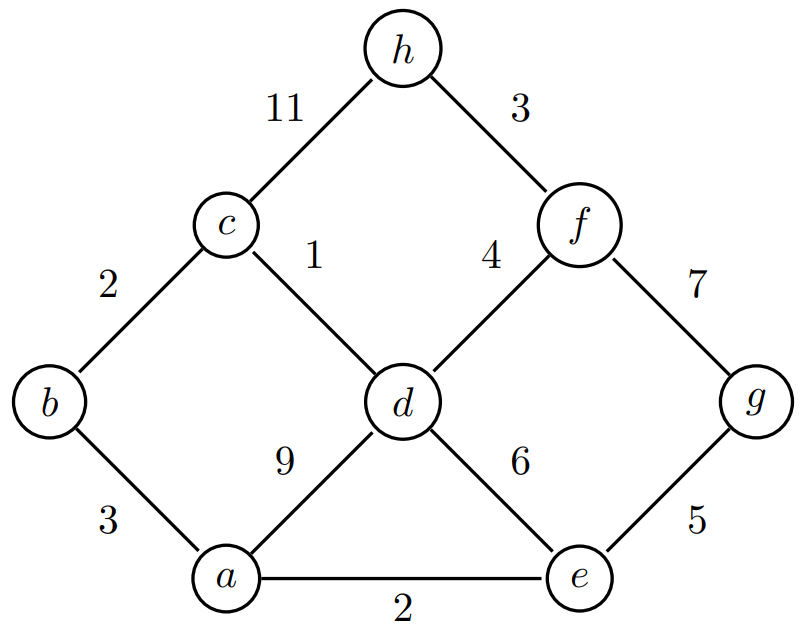
\includegraphics[scale=.5]{3-1.png}
\end{center}
\begin{tabular}{|c|c|c|c|c|c|c|c|c|c|}\hline
				 &     a    &     b    &     c    &     d    &     e    &     f    &     g    &     h    & Chosen Vertex       \\\hline
	Step 1, Prev &          &   (3,a)  & $\infty$ &   (9,a)  &   (2,a)  & $\infty$ & $\infty$ & $\infty$ & e \\\hline
	Step 2, Prev &          &   (3,a)  & $\infty$ &   (8,e)  &          & $\infty$ &   (7,e)  & $\infty$ & b \\\hline
	Step 3, Prev &          &          &   (5,b)  &   (8,e)  &          & $\infty$ &   (7,e)  & $\infty$ & c \\\hline
	Step 4, Prev &          &          &          &   (6,c)  &          & $\infty$ &   (7,e)  &  (16,c)  & d \\\hline
	Step 5, Prev &          &          &          &          &          &  (10,d)  &   (7,e)  &  (16,c)  & g \\\hline
	Step 6, Prev &          &          &          &          &          &  (10,d)  &          &  (16,c)  & f \\\hline
	Step 7, Prev &          &          &          &          &          &          &          &  (13,f)  & h \\\hline
\end{tabular}
\end{enumerate}
\end{document}
